\chapter{Results and Discussion}

\section{Pipeline}
\subsection{Input}
\subsection{Distances}
\subsection{Structure Realization}
\subsection{Evaluation and Visualization}

\begin{itemize}
    \item TM score, GDT\_TS
\end{itemize}
    
\section{Distance predictions}
\subsection{Perceptron}
\subsection{Simple CNN (LeNet)}
\subsection{AlphaFold}
\subsection{Overtraining of the model}
We performed an experiment, to observe how our model behaves with different kinds of data.
First, we initialized the model parameters randomly.
Our primary expectation was that, if we use also randomly generated input and no training, the output will look very randomly as well.
% This expectation is visualized in the Figure (\ref{fig:in_out_dep1}).
    
% \begin{figure}
%     \centering
%     \includegraphics{}
%     \caption{Caption}
%     \label{fig:in_out_dep1}
% \end{figure}
    
Surprisingly, this was not the case in the experiment.

\begin{figure}
    \centering
    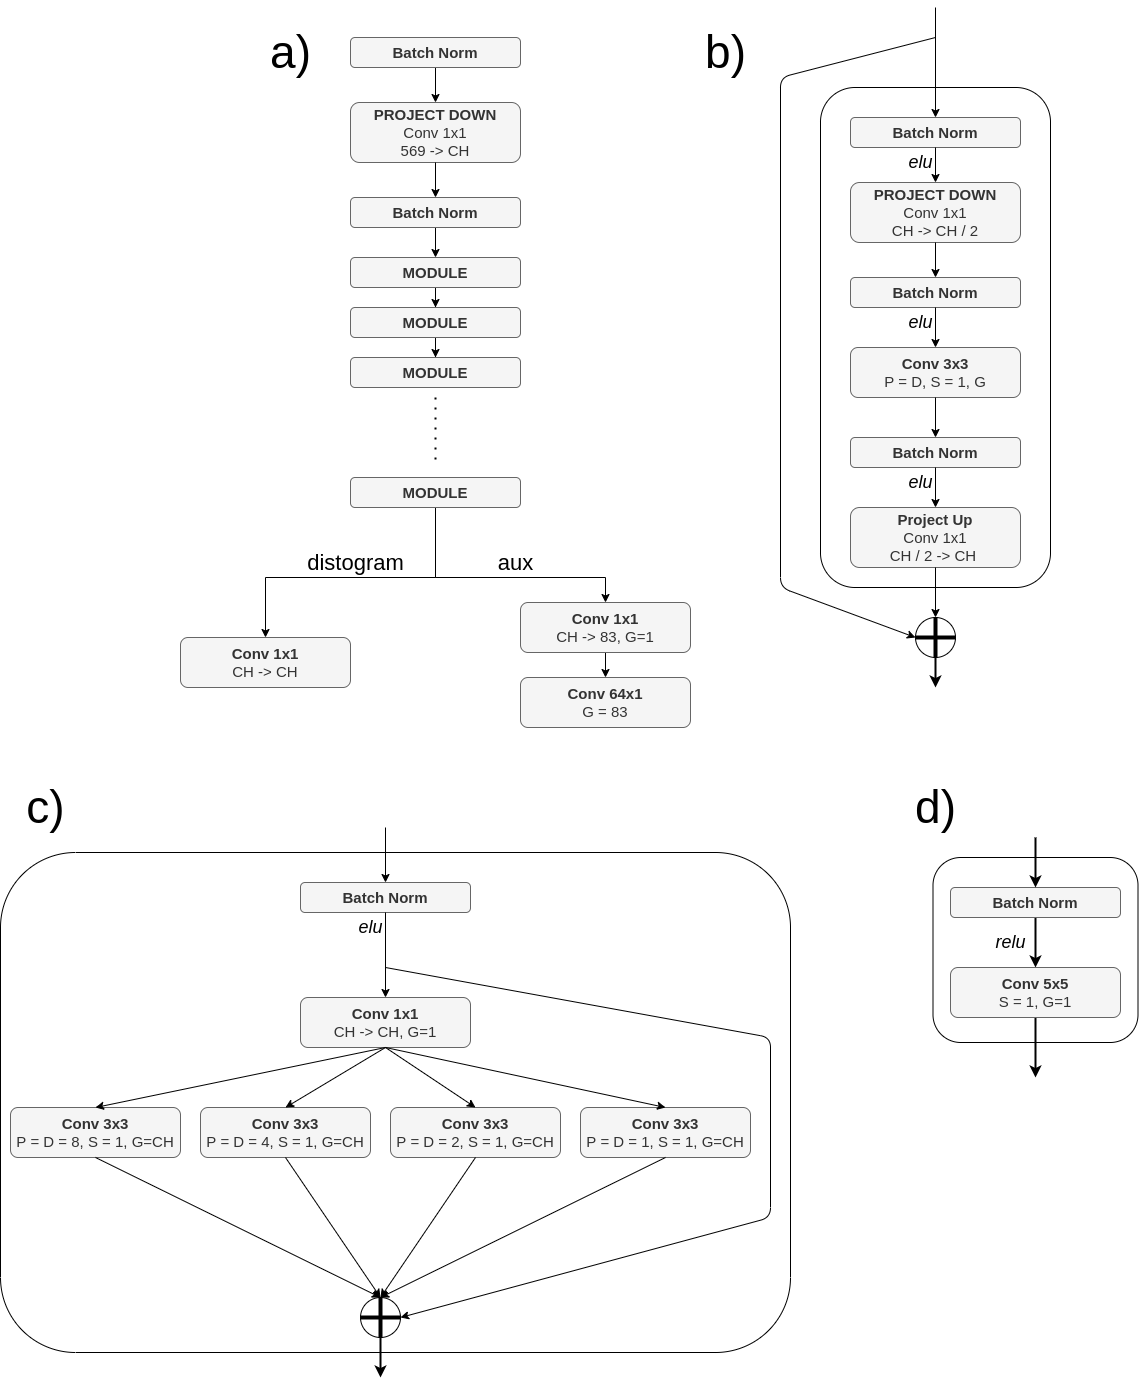
\includegraphics[width=\linewidth]{imgs_tomas/Architectures.png}
    \caption{Neural Network architectures used in training. a) visualizes the diagram of the entire network; b) shows the AlphaFold module, c) is a Inception Resnet module (inspired by Inception module used in GoogleNet) and d) is a simple Convolutional Network}
    \label{fig:architectures}
\end{figure}

Number of parameters:

AlphaFold\_A = 
AlphaFold\_T = 10,745,464
Inception = 1,495,416
ConvNet = 6,654,328

\begin{itemize}
    \item Architecture (Blocks, dilated convolutions, groups)
    \item Number of parameters
    \item Projections (Up, Down) - Conv1x1
    \item Auxiliary losses
\end{itemize}

\begin{figure}
    \centering
    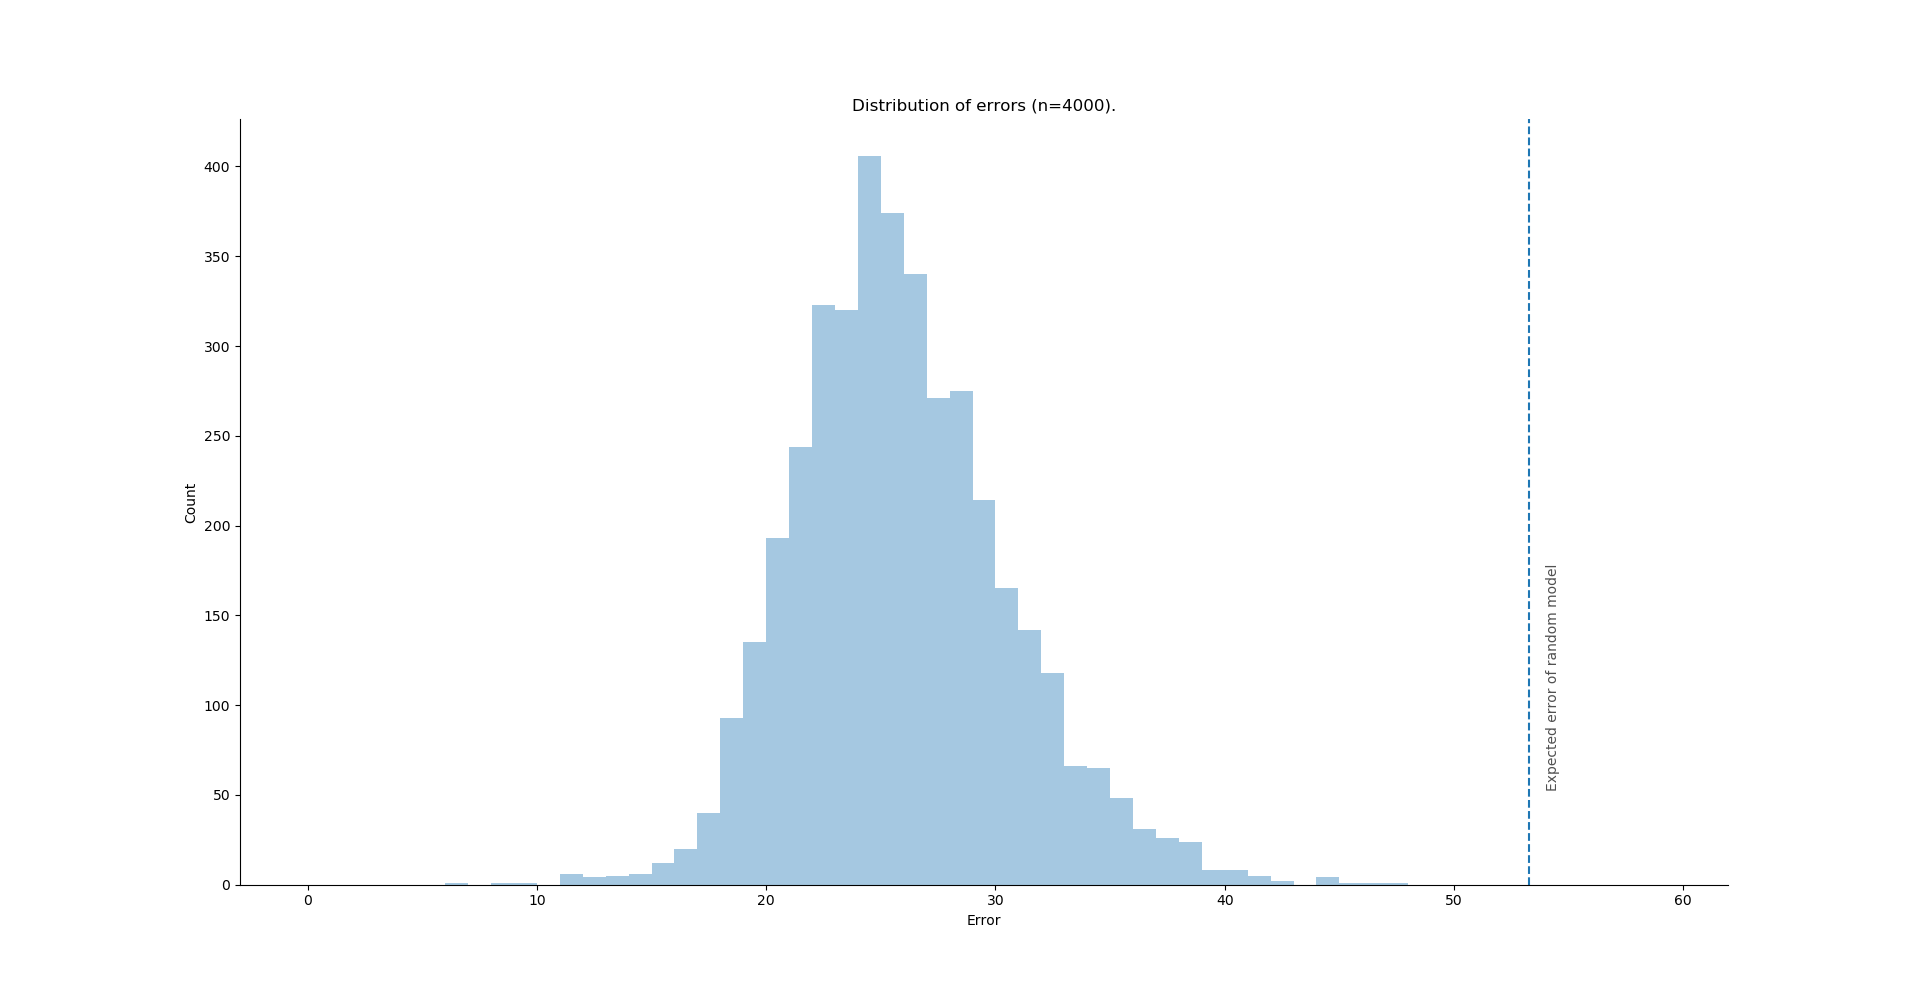
\includegraphics[width=\linewidth]{imgs_andy/error_distribution_200430m93s4000.png}
    \caption{Caption}
    \label{fig:error_dist}
\end{figure}

\begin{figure}
    \centering
    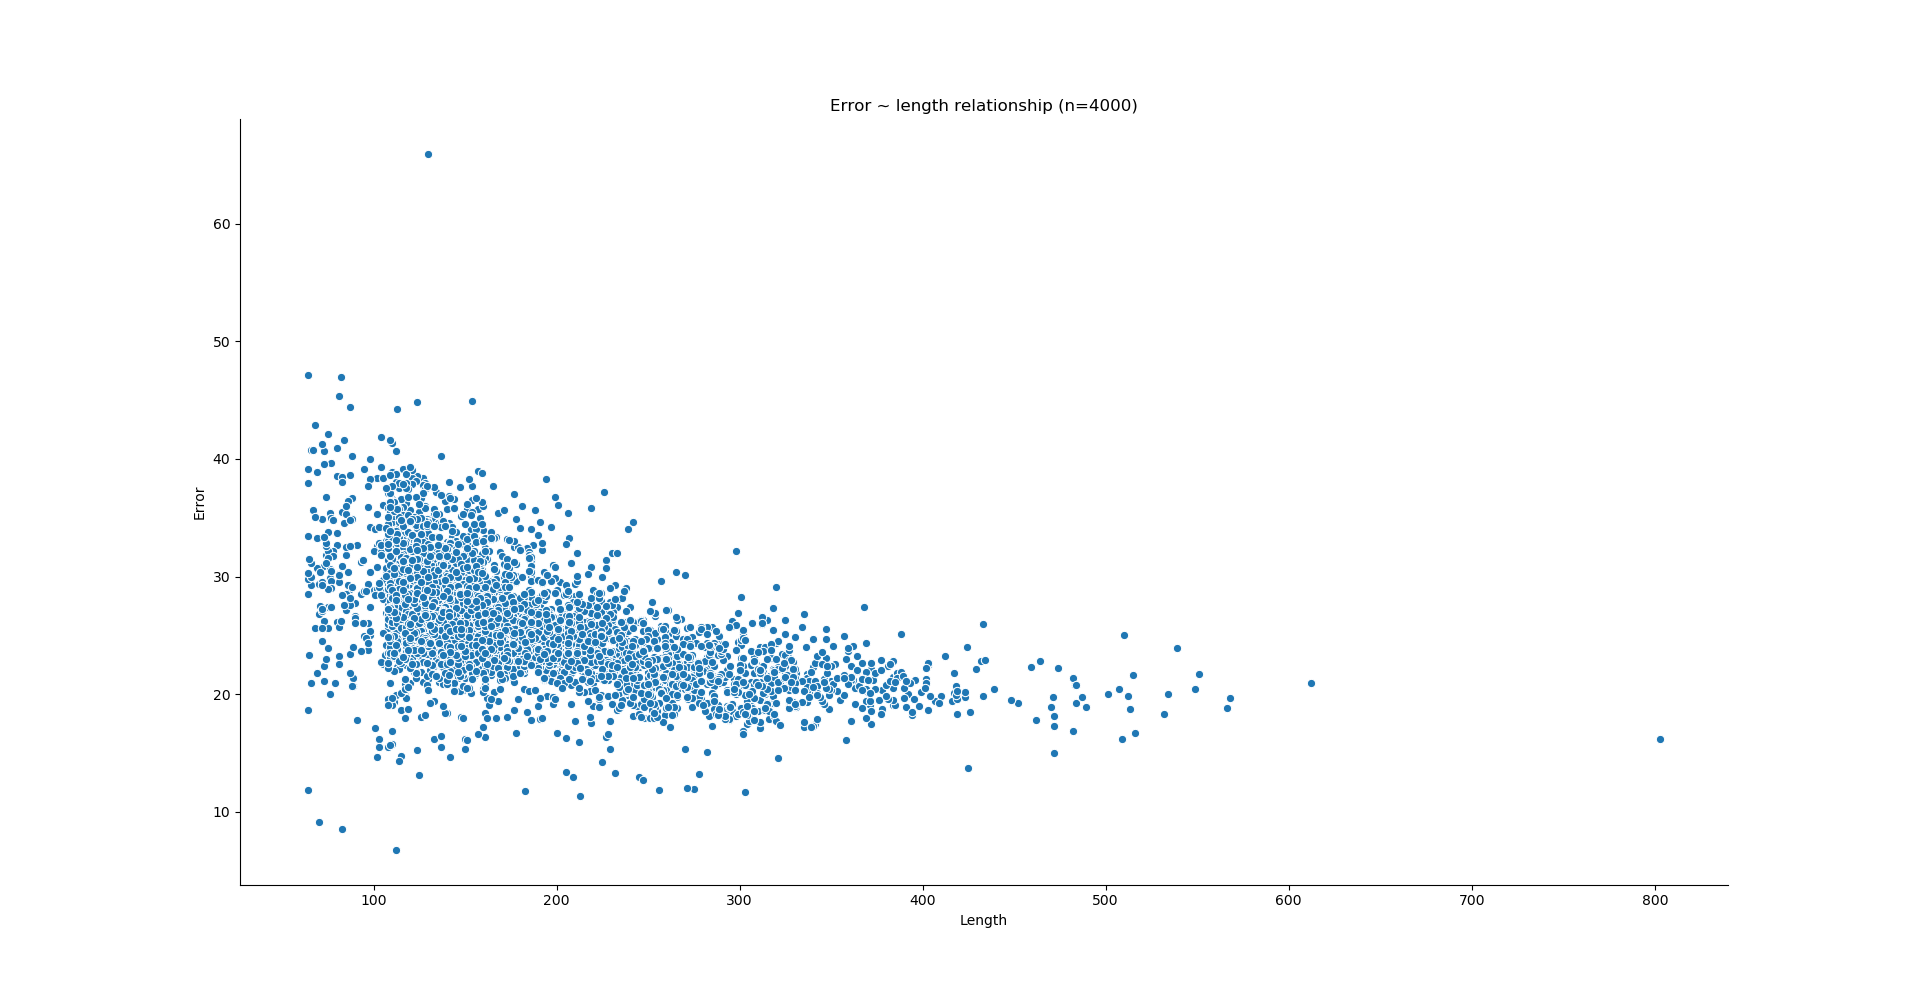
\includegraphics[width=\linewidth]{imgs_andy/error_length_200430m93s4000.png}
    \caption{Error - length relationship}
    \label{fig:err_len}
\end{figure}

\begin{figure}
    \centering
    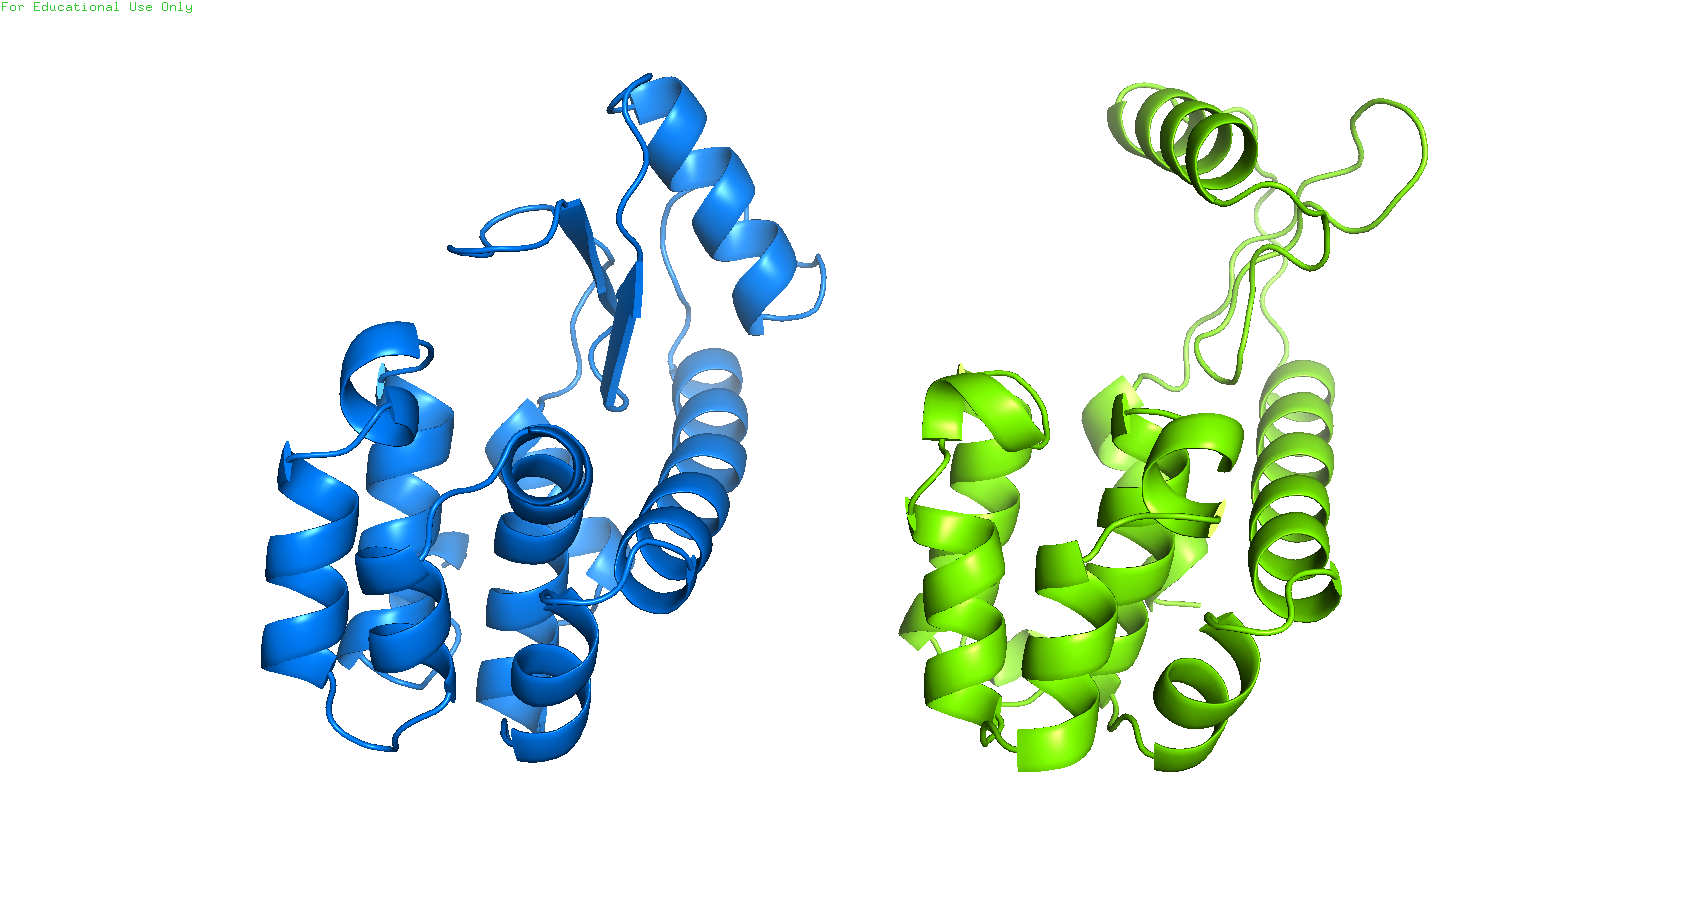
\includegraphics[width=\linewidth]{imgs_andy/139lA00_real_pred_3D_v2.png}
    \caption{Comparison of real vs. predicted 3D structure}
    \label{fig:real_pred}
\end{figure}

\begin{figure}
    \centering
    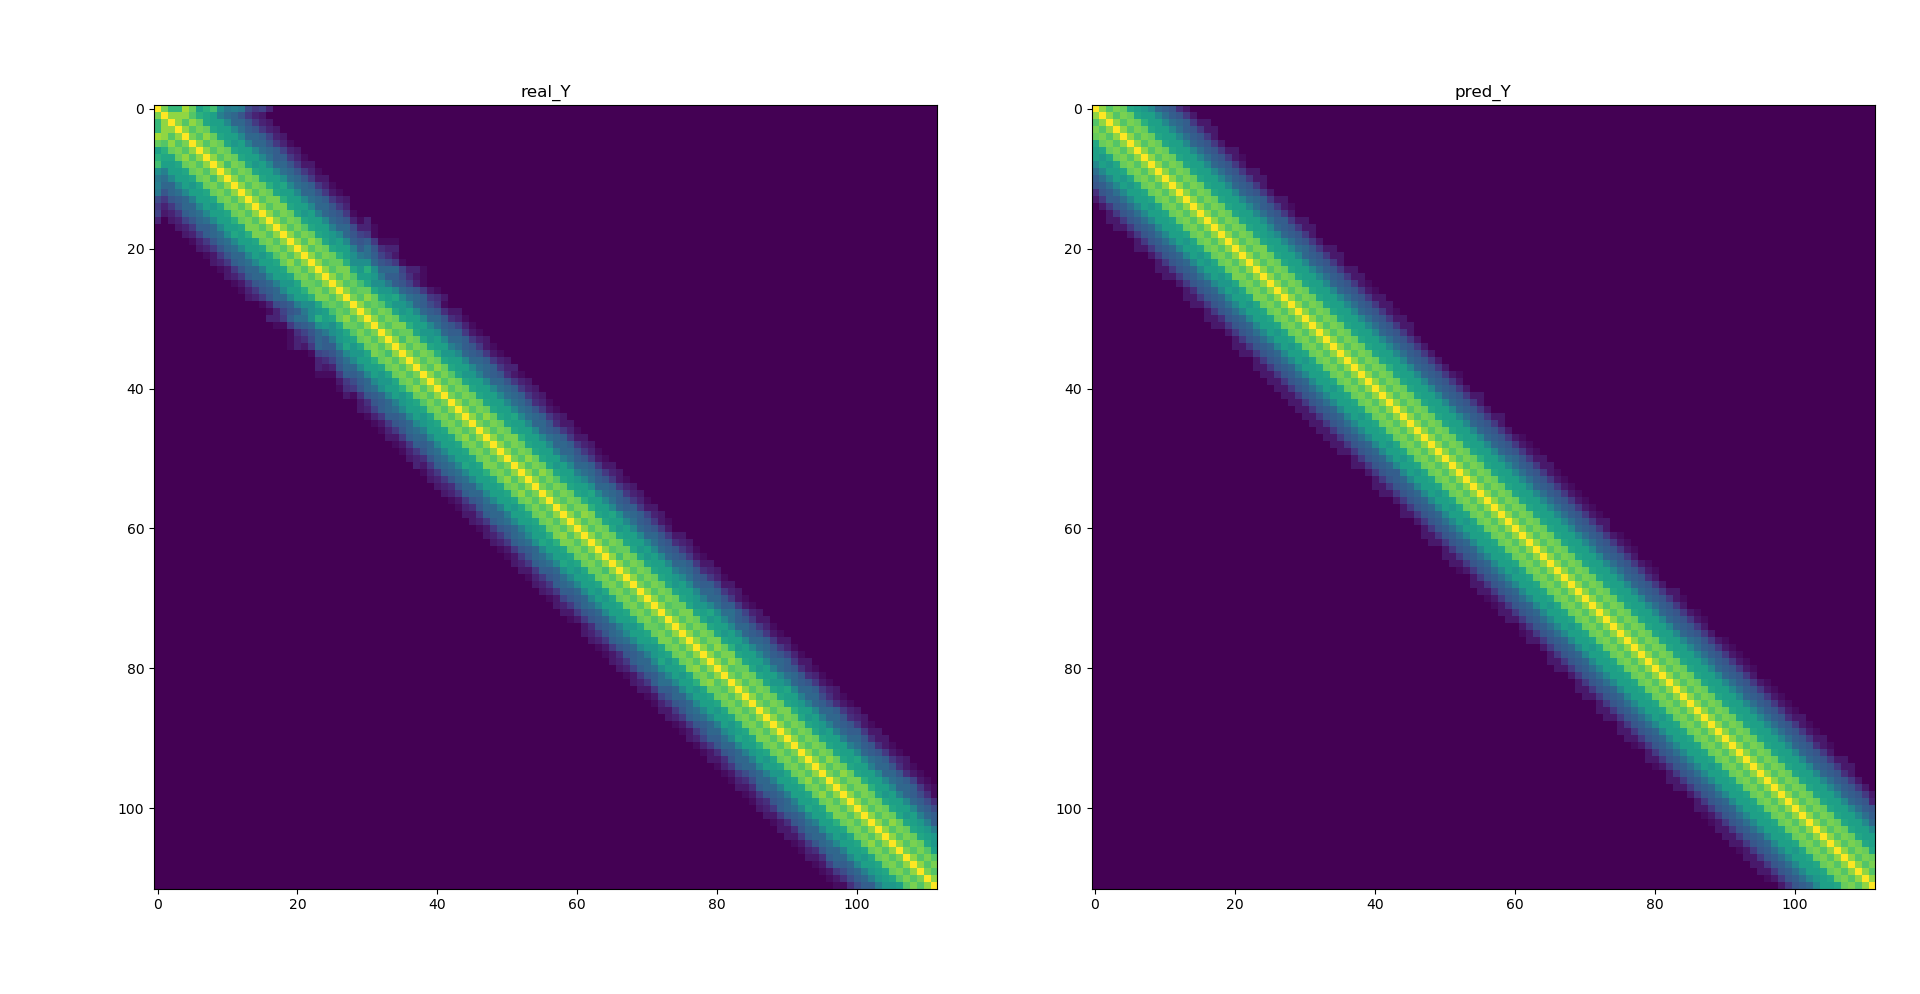
\includegraphics[width=\linewidth]{imgs_andy/2fxmB00_best_prediction.png}
    \caption{Best prediction}
    \label{fig:best}
\end{figure}

\begin{figure}
    \centering
    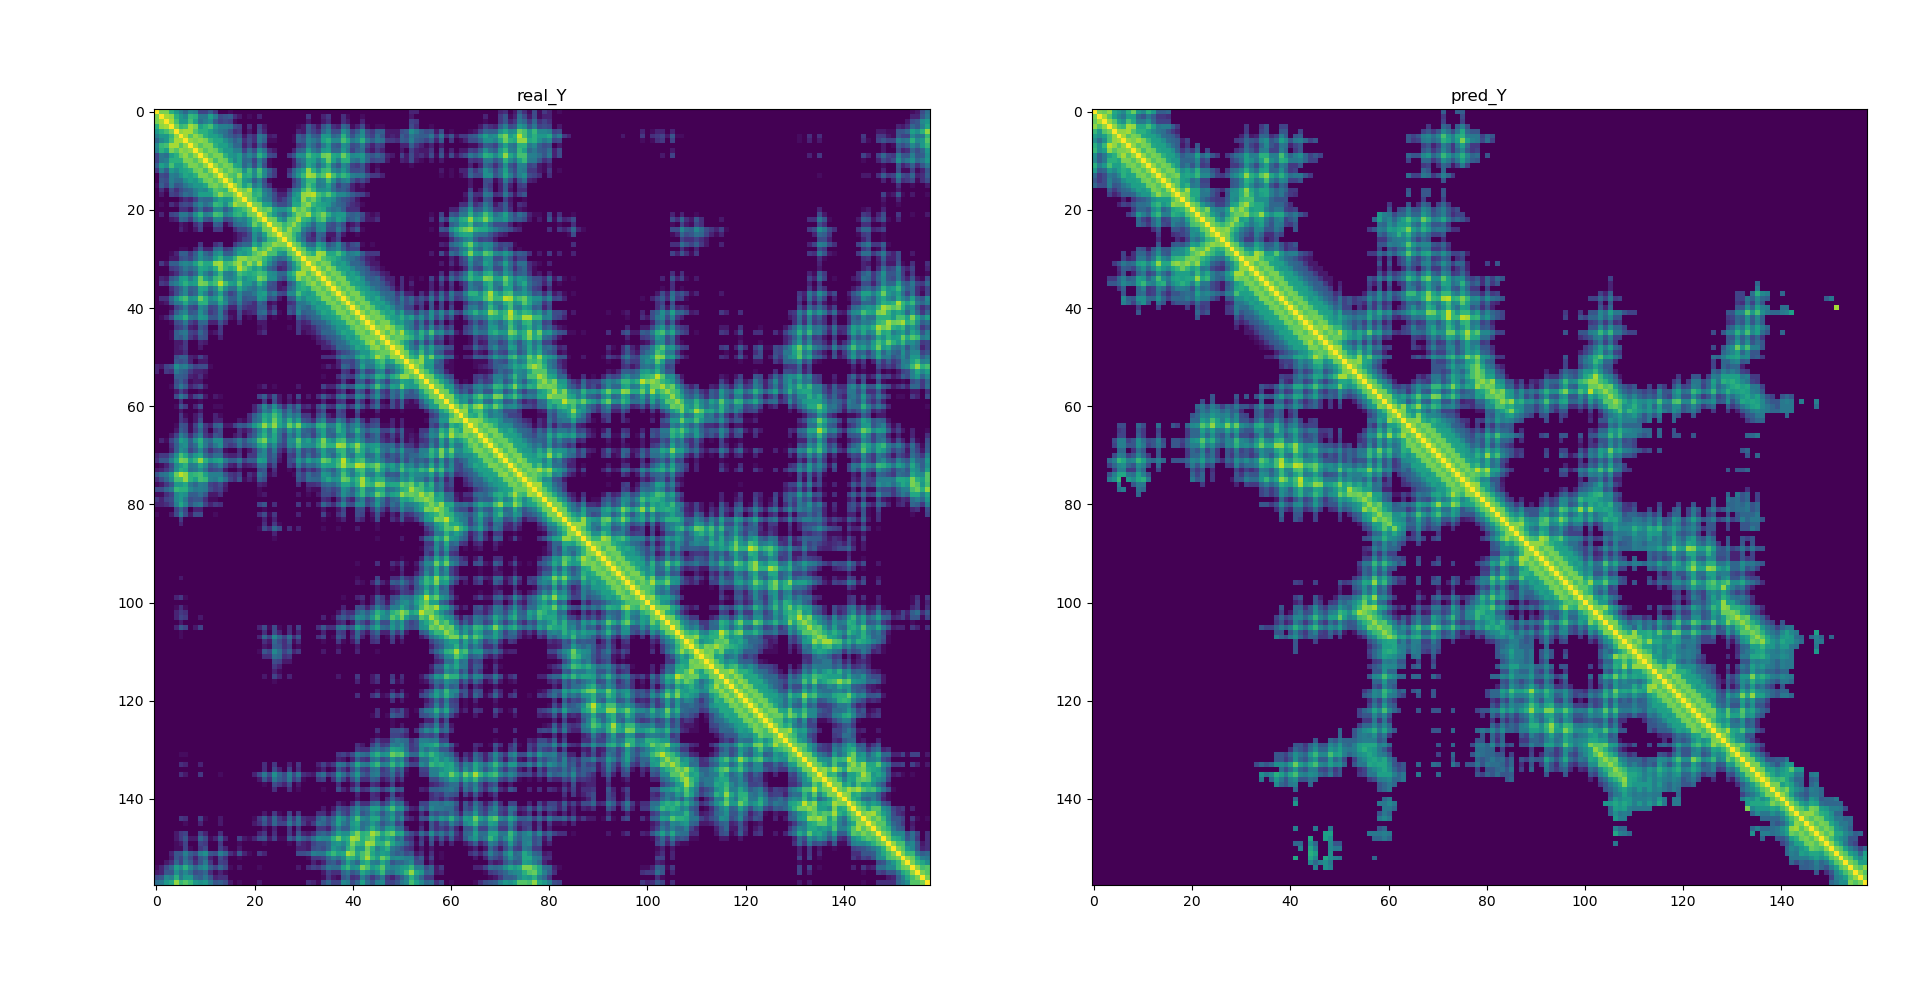
\includegraphics[width=\linewidth]{imgs_andy/1mdbA01_median_prediction.png}
    \caption{Median prediction}
    \label{fig:median}
\end{figure}

\begin{figure}
    \centering
    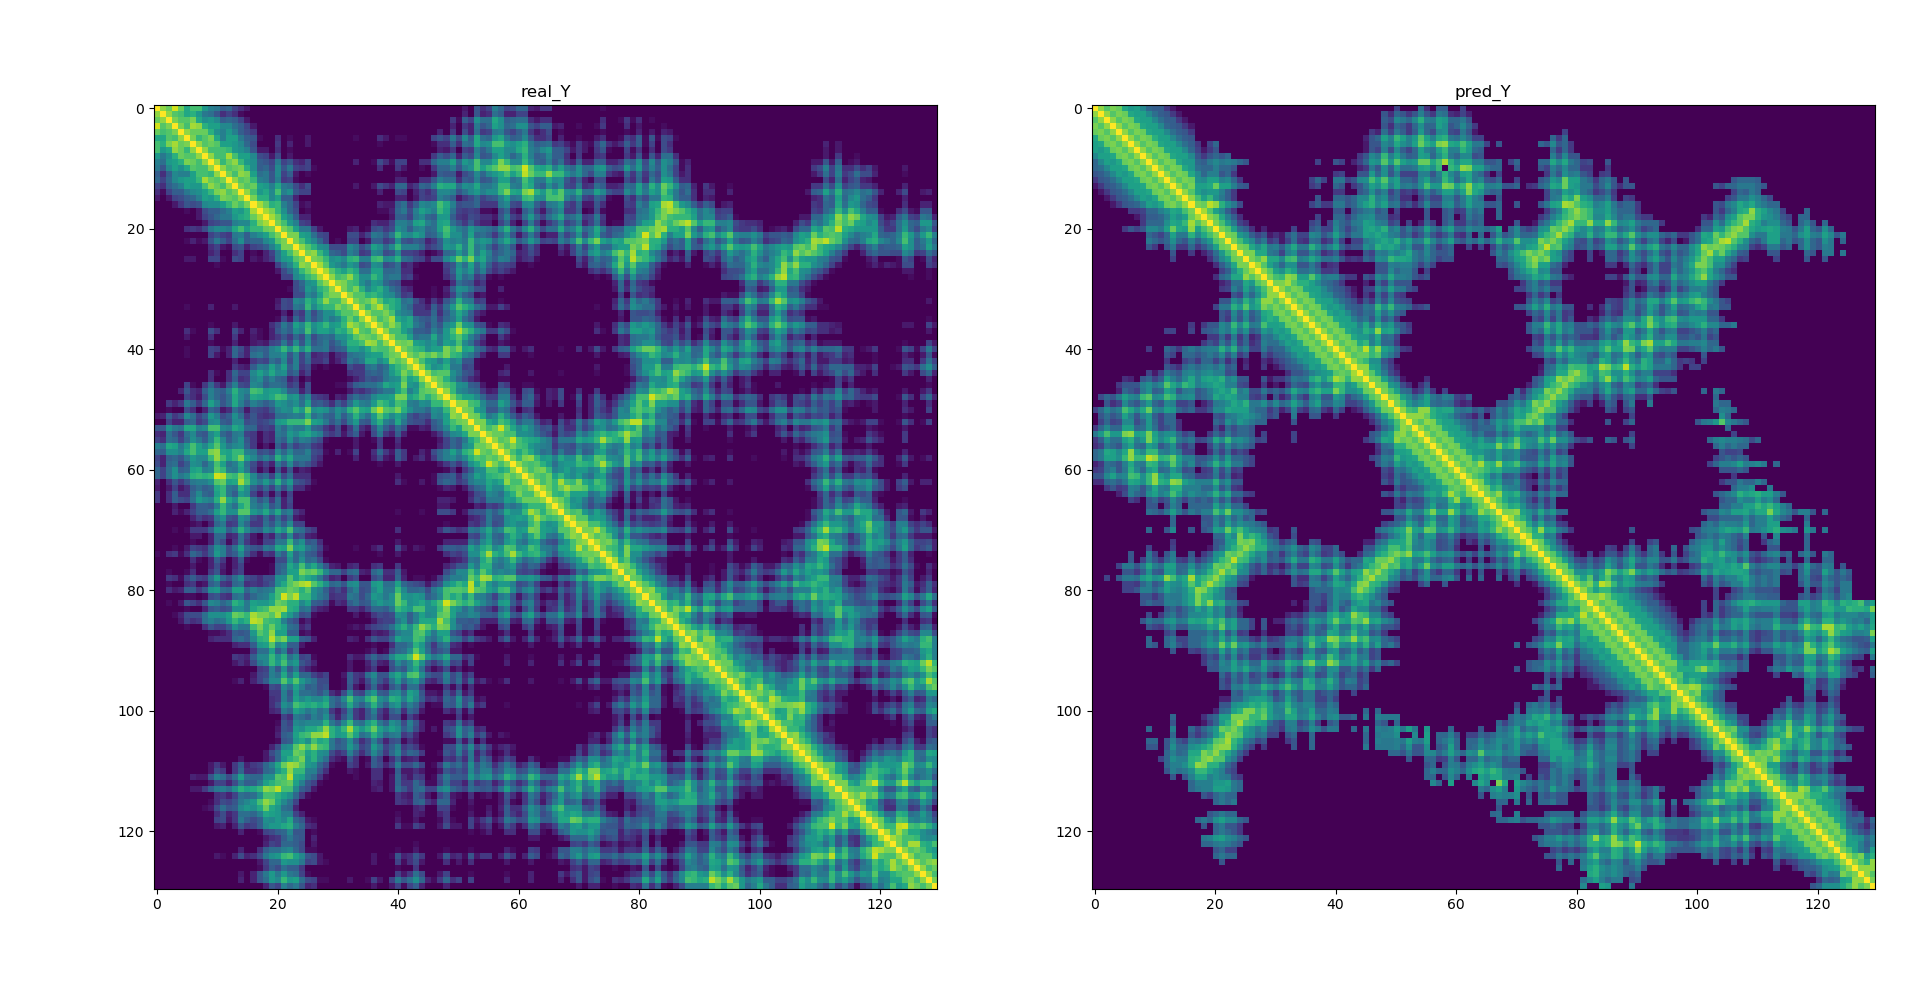
\includegraphics[width=\linewidth]{imgs_andy/3kitJ00_worst_prediction.png}
    \caption{Worst prediction}
    \label{fig:worst}
\end{figure}

\section{Structure Realization}

\subsection{Gradient Descent Based Structure Realization}

\begin{figure}
    \centering
    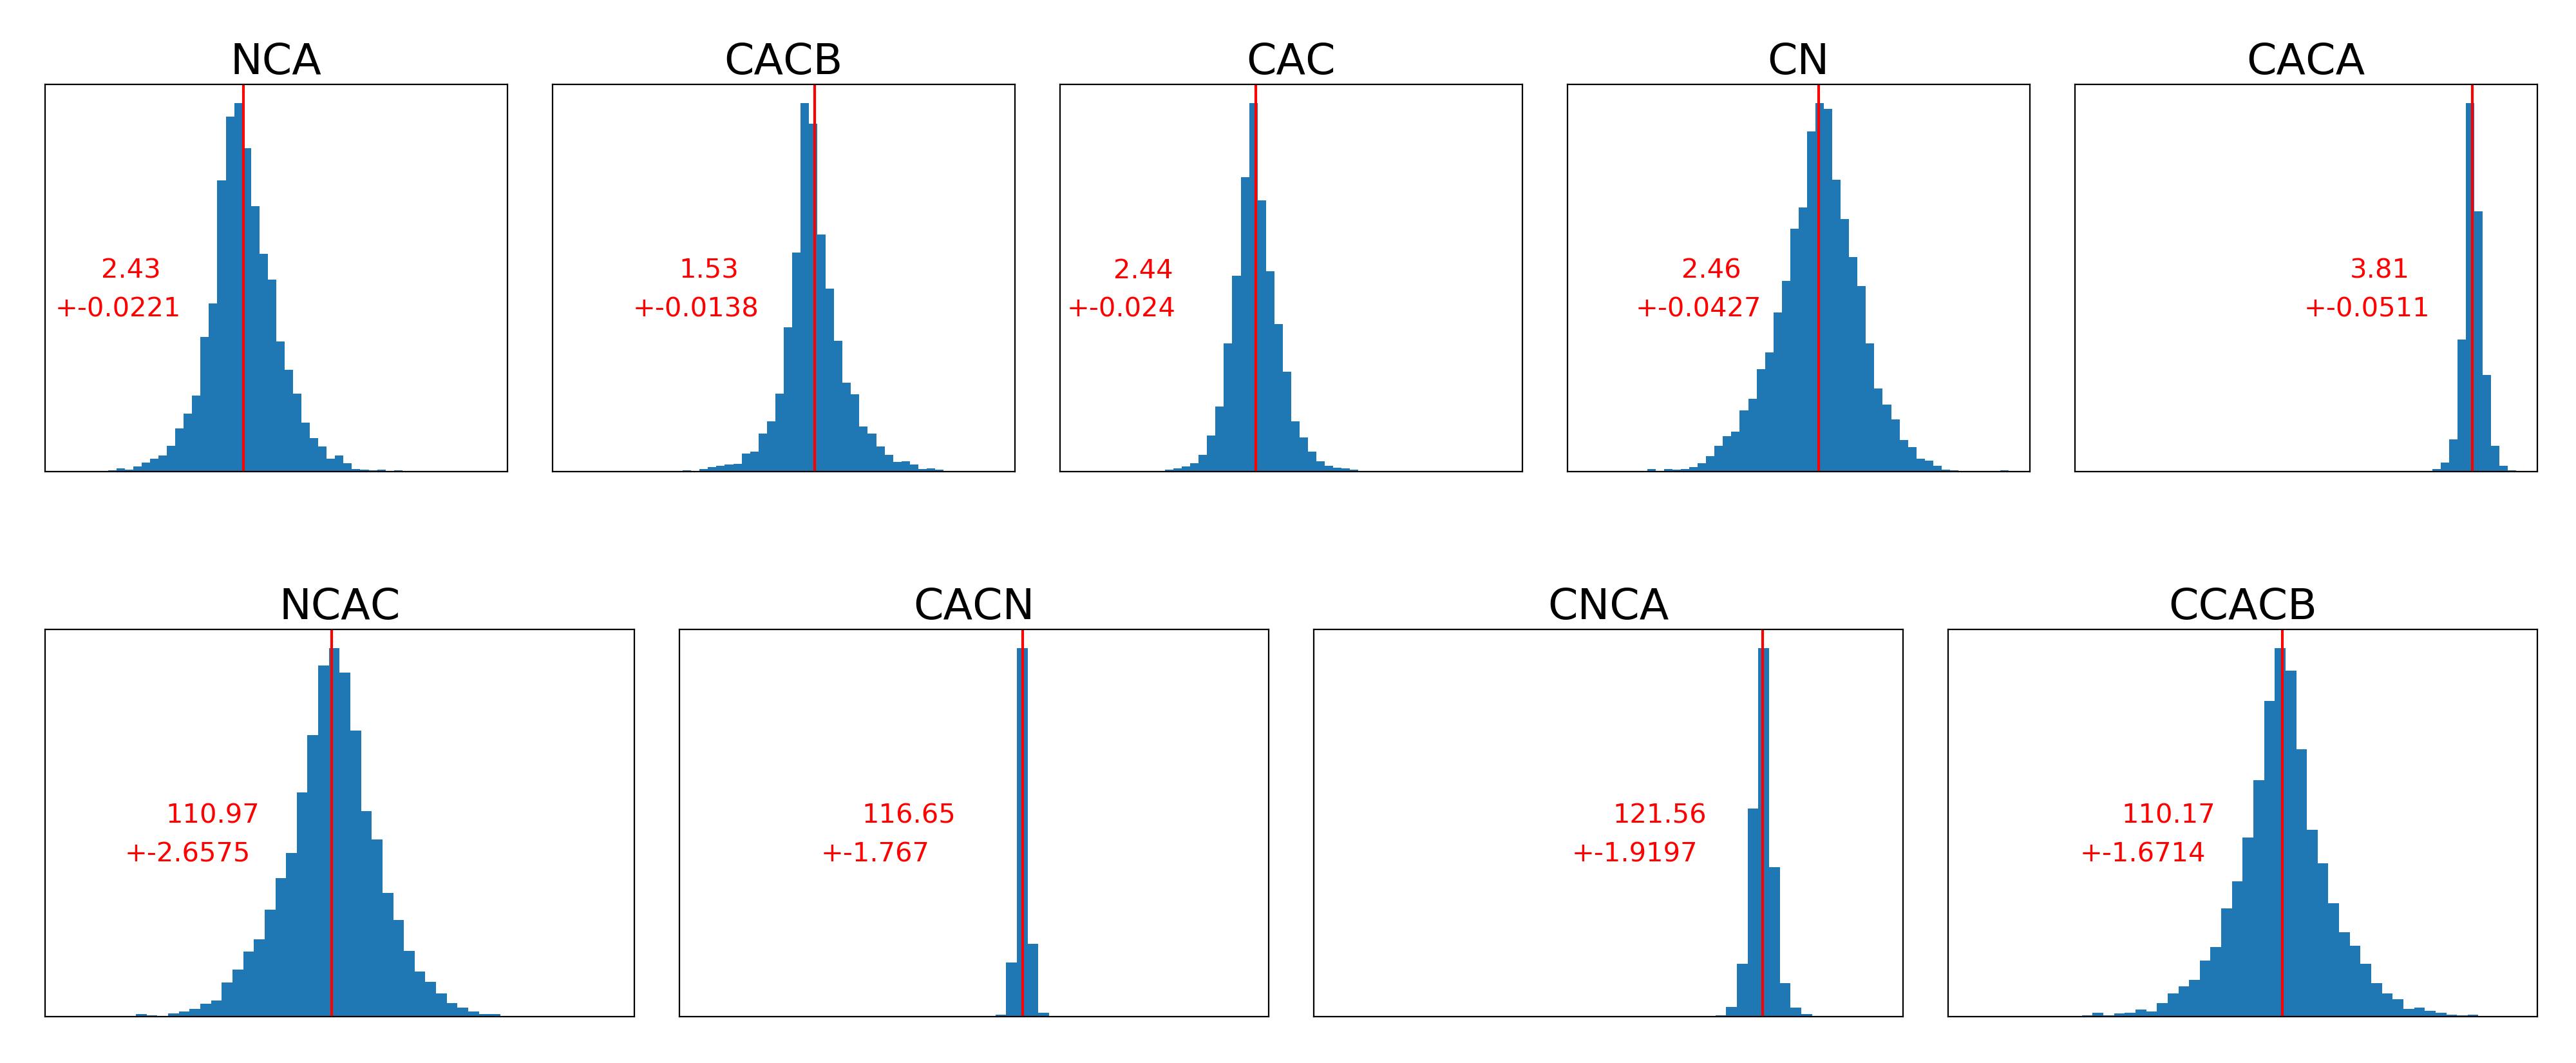
\includegraphics[width=\linewidth]{imgs_tomas/inter_data.png}
    \caption{Inter-atom distance distributions (top row) and angles defined by three consecutive atoms in a plane (bottom row) calculated from 50 protein structure downloaded from PDB. The red line represents the mean of the distribution, together with the first number in red text. The second number is the standard deviation}
    \label{fig:interresidue}
\end{figure}

\begin{figure}
    \centering
    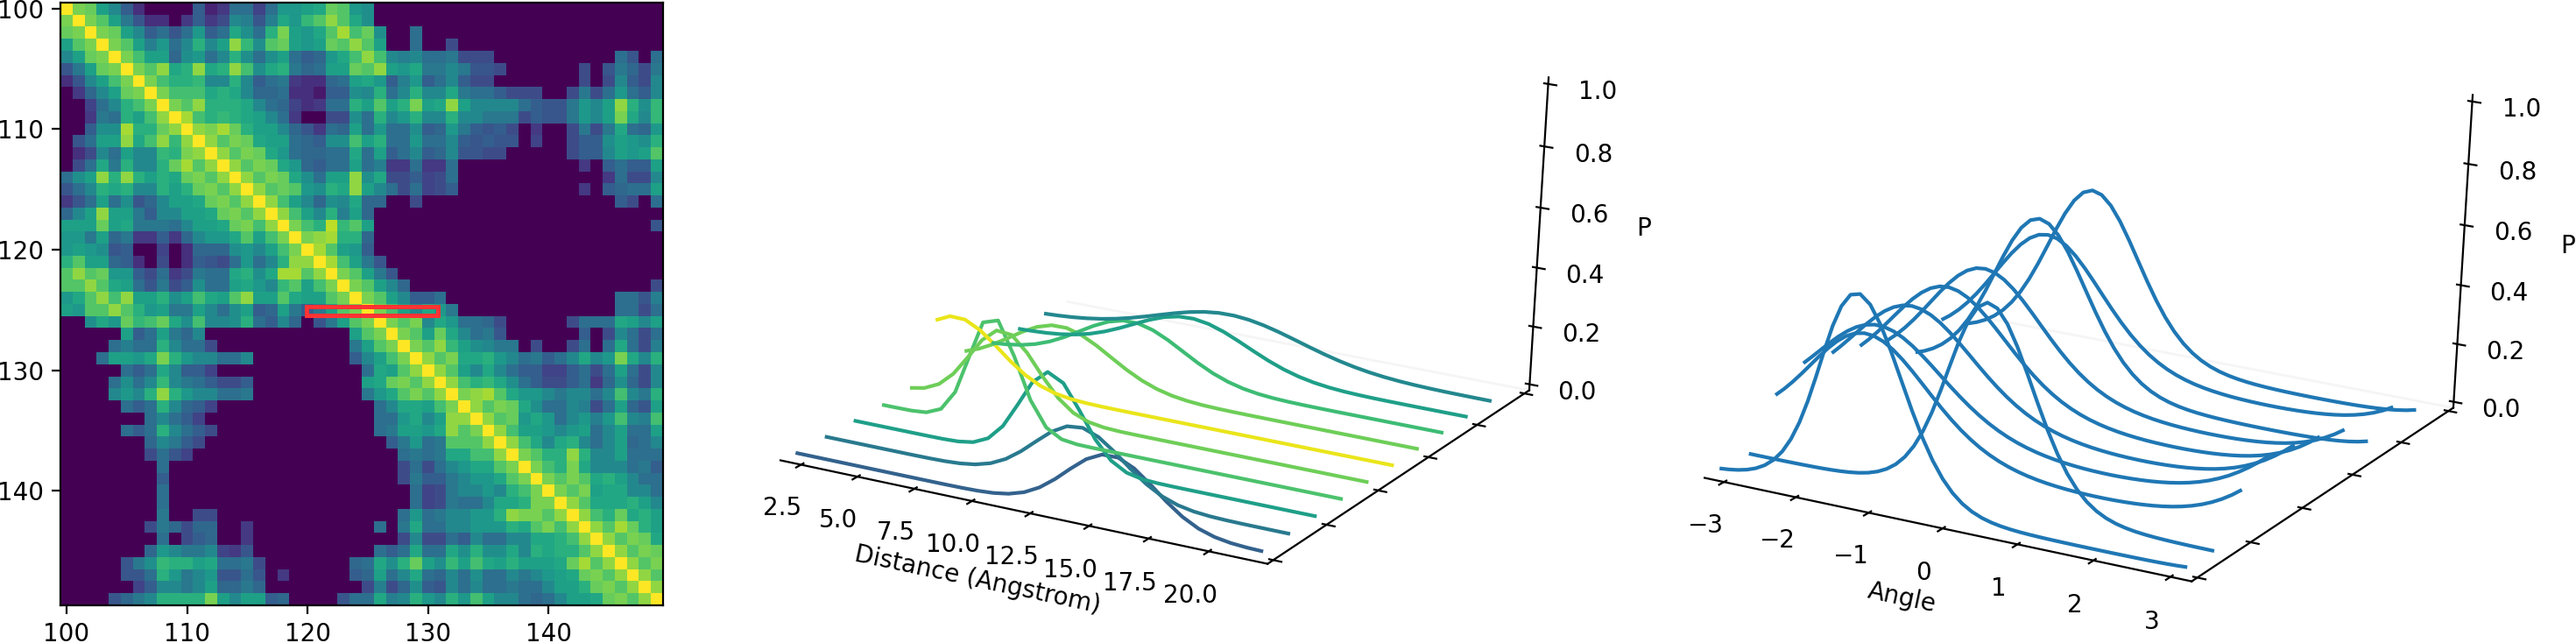
\includegraphics[width=\linewidth]{imgs_tomas/norm_histograms.png}
    \caption{Fitted normal distributions to the distance histograms (middle) and von Mises distributions to the angle histograms (right) to a small region of domain 16pkA01}
    \label{fig:distributions}
\end{figure}

In order to implement the model of protein geometry, one has to treat the distances between neighboring atoms in the backbone as constants, together with the angles of 3 consecutive backbone atoms. We analyzed coordinates of 50 randomly selected proteins and calculated these distances and angles; the results are shown in Figure \ref{fig:interresidue}. The means of the distributions were used in the creation of the protein geometry.

For a given structure we generated 1000 unique random initial states by sampling from the von Mises distributions fitted to the histograms. The individual distributions are depicted on Figure \ref{fig:distributions}. From each angle distribution (right of the Figure \ref{fig:distributions}) one value was picked. The normal distance distributions (Figure \ref{fig:distributions} - middle) were used for the calculation of the loss function - see Equation \ref{eq:dist_pot}.

For each torsion angle initiation we let the algorithm run for 1000 iterations. However, after every 200 iterations the algorithm picked the best structure (according to the loss) and continued the optimization with decreased learning rate (by a factor of 10).

The initial parameters were chosen by visually exploring the learning curves of 3 random states. The grid search was composed of combination of parameters:

$$learning~rate = [0.1, 0.05, 0.01. 0.005, 0.001]$$
$$momentum = [0.1, 0.3, 0.5, 0.7, 0.9]$$


\subsection{Inter-residue Contacts + Secondary structure based Structure Realization}


\section{Comparison with other methods}
\subsection{Distances}
\subsection{Structures}

\section{What next?}

\subsection{Regarding Input Data}
what to do when the protein does not have enough similar sequences in the database?
NEFF

PLMC might not converge. What are the reasons for this and how should we handle it.

Optimization of the input pipeline is needed.
HHblits and Psiblast both do a sequence search and MSA.
Ideally we would like to do this just once and then from MSA compute the PSSM and potts models.
Although it might be beneficial to do it like it is, because the input features will be less correlated to each others.

It might be beneficial to include calculated limits of the physical distance of 2 aminoacids.
For example, we know that 2 aminoacids next to each other are 3.8A away.
Similarly, 2 aminoacids at position $i$ and $i+2$ are ???5.6???A away.
For position $i$ and $i+3$ this starts t be interesting, but calculating the maximum distance and the minimum distance should be relatively easy.

Refactoring pipeline to be truly reproducible.

Using more covariance data modelling approaches, not just PSSM and potts, but also PSICOV and Bayesian networks.

\subsection{Regarding Neural Networks}
Neural networks could be modified to predict parameters of some distribution of distances.
In currect setting we are predicting distrogram characterized by 32 numbers.
If we would be able to identify some reasonable parametric distribution for distances, these could be used instead of the distrogram, reducing the number of parameters of the network and making the formulation closer to some theorethical formulation related to protein than very general.

Use accumulating gradients. This would allow to train on bigger batches than is the memory limit of the GPU and also would allow to train on multiple GPUs.
% https://medium.com/huggingface/training-larger-batches-practical-tips-on-1-gpu-multi-gpu-distributed-setups-ec88c3e51255

\subsection{Regarding Structure Realization}

Even though the algorithm for optimizing structure works, it is highly dependant on the choice of hyperparameters, which might not be ideal for every domain. The authors of AlphaFold did not use gradient descent for optimization but a more advanced method - L-BFGS (Limited memory Broyden–Fletcher–Goldfarb–Shanno) which is a method which resembles the second order optimization by estimating the Hessian matrix (matrix of second derivatives). The method does not pick directions where the loss function changes the fastes, but rather where the gradients change the fastest. This results in more reasonable especially and the convergence is usually reached in smaller number of steps. The biggest downside of the method is, that it is slow and tends to get stuck in saddle points of the loss function \cite{nn_dl}.